\chapter{Marco Teórico} \label{chap:marcoteorico}

En el siguiente capitulo se pondrá al alcance del lector las bases teóricas y los conocimientos necesarios para poder entender las diferentes terminologías utilizadas en el trabajo de investigación realizado.

Se tratará de dar un enfoque simplificado de temas como: ¿que es el sensado remoto?, ¿que es el Aprendizaje Automatico?, descripción y desarrollo de Algoritmos de optimización, validación de modelos, Computer Vision.

Para finalizar se expondra la arquitectura, entrenamiento y reconocimiento de objetos a traves de  redes neuronales convolucionales y clasificadores.

\section{Sensado Remoto}\label{sec:sensadoremoto}

En esta sección desarrollaremos el principal enfoque de este trabajo que son las imágenes satelitales; como se forman, rangos de bandas, instrumentos utizados y datos con los cual se trabaja.

\subsection{Teledetección}\label{sub:teledeteccion}

Para comenzar a introducir el concepto de imagen satelital debemos saber como esta formada la misma, es por esto que vamos a desarrollar el concepto de \textit{teledetección}.

La teledeteccion o sensado remoto tambien llamado es el proceso que nos permite obtener una imagen de la superficie terrestre de forma remota, es decir sin estar en contacto con ella. Una imagen satelital es una representación de estos datos reflejados por la superficie terrestre que son captadas por un sensor que se encuentran a bordo de un satélite artificial (ver fig \ref{Fig:teledeteccion}).

La teledeteccion no es mas que la detección de propiedades relevantes del entorno; esta capacidad no es despreciable, nos permite desarrollar aplicaciones practicas con un impacto cada ves mayor \citep{percepcion}. 

En general la teledetección es la medición de energía emanada de la superficie terrestre. Existen diferentes fuentes de energia; si la fuente de energía es el sol entonces lo llamamos \textit{teledetección pasiva}, si la energia medida no es emitida por el Sol, es decir es emitida por un sensor, llamamos \textit{teledetección activa}, como por ejemplo los sensores de radar que funcionan en el rango de microondas.

Los componentes basicos de un sistema de teledetección incluye lo siguiente \citep{chuvieco}:
\begin{itemize}
\item \textit{Fuente de energia}: es la radiación electromagnética que capta el sensor; como mencionamos anteriormente puede tratarse de una fuente pasiva o activa.

\item \textit{Cubierta terrestre}: rasgos naturales o relizados por el hombre, ejemplo construcciones, que refleja el sensor.

\item \textit{Sistema Sensor}: esta computesto por, camaras, radar, etc; y la plataforma en la que esta puesto (satelite, avion, globo);  capta la energía proveniente de la tierra y la almacena o envía al sistema de recepción.

\item \textit{Sistema de Recepción}: sistema encargado de recibir la información proveniente del sensor y almacenar en un formato apropiado para luego ser distribuido a los usuarios.

\item \textit{Interprete}: encargado de manipular los datos de acuerdo a la temática de interes (agricultura, catastro, etc), es decir aplica diferentes niveles de procesamiento sobre los datos crudos obtenidos por el sensor.

\item \textit{Usuario Final}: es el consumidor final de la imagen adquirida.
\end{itemize}

\begin{figure}[H] \centering
  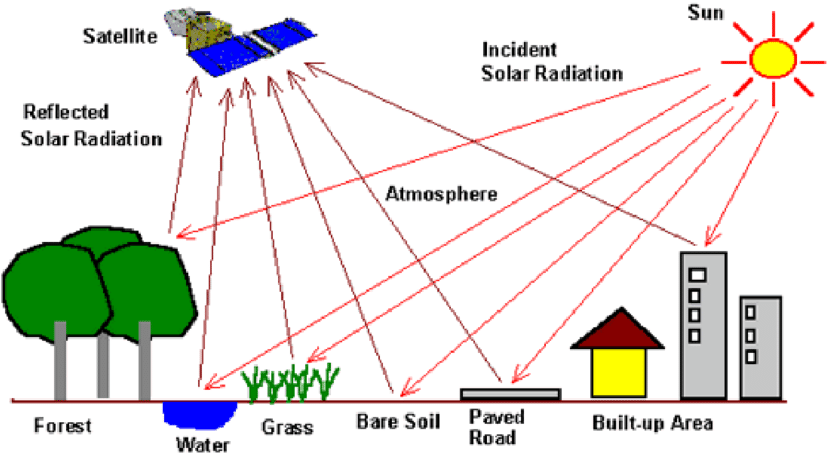
\includegraphics[height=8cm,keepaspectratio=true,clip=true]{imagenes/MarcoTeorico/teledeteccion.png}
  \caption{Sensado Remoto. Navarrete, Edison, Laubacher, Gerard}\label{Fig:teledeteccion}
\end{figure}

\subsubsection{Tipos de Sensores}
\begin{itemize}
\item \textbf{sensores pasivos}: son aquellos que reciben las señales emitidas naturalmente que fueron reflejadas por los objetos. Estas señales son a partir de la radiación solar natural. Este tipo de sensores son  usados mayormente en apliacaciónes de evaluación de recursos naturales. Ejemplo: ASTER, MODIS, VIIRS, LandSat.

\item \textbf{sensores activos}: son aquellos que emiten radiación dirigida hacia un objetivo especifico, esta raciación reflejada del objeto es detectada y medida por el sensor. Ejemplo: Radar, Sonar.
\end{itemize}

\subsubsection{Espectro electromagnético}

El espectro electromagnético se denomina al conjunto de todas las longitudes de onda \citep{chuvieco}. Las ondas electromagnéticas cubren una amplia gama de frecuencias o de longitudes de ondas y pueden clasificarse según su principal fuente de producción. 
Las regiones utilizadas para la observación remota de la tierra son:
\begin{itemize}
\item Espectro visible (0.4 - 0.7 µm): rango de frecuencias del ojo humano; máxima radiación solar. Subdividido en tres bandas: Rojo (0.6 - 0.7 µm), Verde (0.5 - 0.6 µm) y Azul (0.4 - 0.5 µm).

\item Infrarrojo cercano (0.7 - 1.1 µm): denominado IR fotográfico o reflejado; energía solar que reflejan los cuerpos. Comportamiento similar al espectro visible.

\item Infrarrojo medio (1.1 – 8 µm): se entremezclan radiación solar y emisión; la atmósfera afecta sensiblemente: aprovechado para medir concentraciones de vapor de agua, ozono, aerosoles, etc.

\item Infrarrojo térmico (8 - 14 µm): radiaciones emitidas por los propios cuerpos; se puede determinar la Temperatura de un cuerpo (IRtérmico). Se puede disponer de imágenes a cualquier hora del día.

\item Microondas (1mm-1m): Interés creciente de la Teledetección en esta banda; las perturbaciones atmosféricas son menores y es transparente a las nubes. Se suelen utilizar sensores activos. 

\end{itemize}

\begin{figure}[H] \centering
  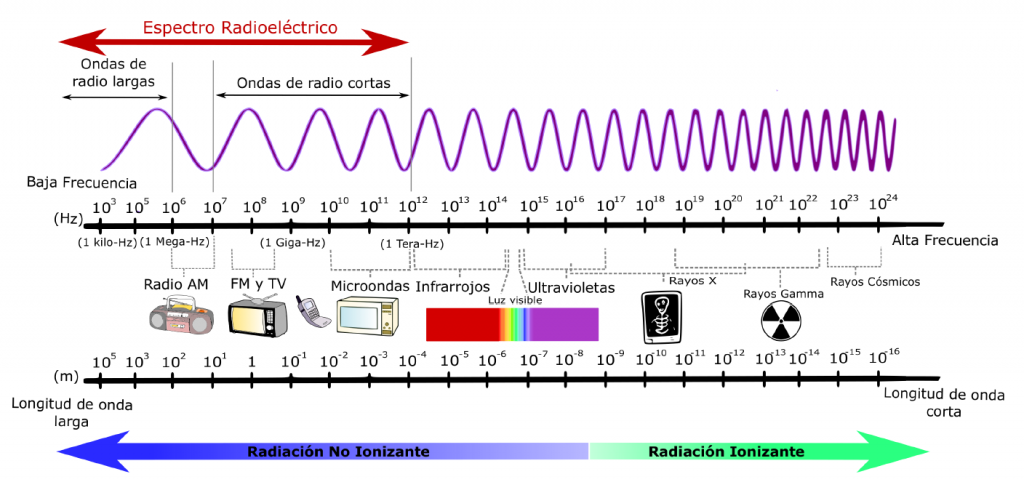
\includegraphics[height=8cm,keepaspectratio=true,clip=true]{imagenes/MarcoTeorico/espectro-electro.png}
  \caption{Espectro electromagnético \citep{https://iie.fing.edu.uy/proyectos/esopo/eem/}}\label{Fig:espectro-electromagnetico}
\end{figure}


\subsubsection{Resolución}
Unas de las características de los sensores son el tipo de imagen que proporiciona; estas características vienen definidas por el timpo de resolución. Estas resoluciónes la podemos definir de la siguiente manera:

\begin{itemize}
\item \textbf{Resolución Espacial}: distancia que corresponde a la unidad mínima de información incluida en un píxel. A menor tamaño de píxel mayor sera la resolución espacial, esto quiere decir que el sensor tendrá mayor detalle de los objetos.

\begin{figure}[H] \centering
  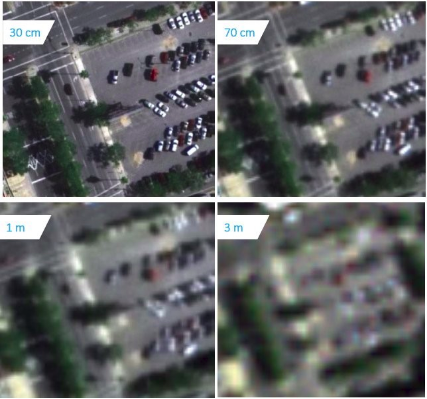
\includegraphics[height=8cm,keepaspectratio=true,clip=true]{imagenes/MarcoTeorico/resolucion.png}
  \caption{Resolución espacial \citep{https://iie.fing.edu.uy/proyectos/esopo/eem/}}\label{Fig:resolucion-esp}
\end{figure}

\item \textbf{Resolución Espectral}: la resolución espectral especifica el numero y la anchura de las badas espectrales que puede ser discrimidadas por el sensor.
\begin{figure}[H] \centering
  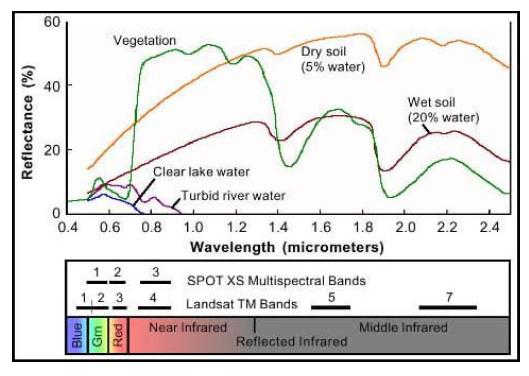
\includegraphics[height=8cm,keepaspectratio=true,clip=true]{imagenes/MarcoTeorico/resolucion_espectral.jpg}
  \caption{Resolución espectral \citep{http://laotraopinion.net/wp-content/uploads/poder-de-resolucion-espectral.jpg}}\label{Fig:resolucion-espectral}
\end{figure}

\item \textbf{Resolución Radiometrica}: indica el numero de bits utilizados para expresar los datos recogidos por el sensor. Mayormente cuando es mas grande el número de niveles mayor es el detalle con la cual se podrá expresar dicha información. Ejemplo los sensores Landsat (5 y 7) utilizan 8 bits lo que da 2**8= 256 niveles de energía que pueden ser captados.
\begin{figure}[H] \centering
  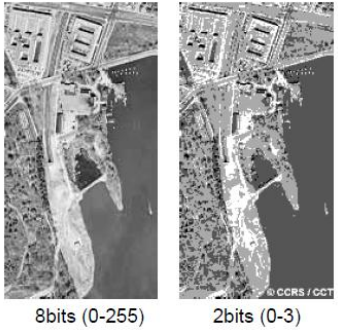
\includegraphics[height=8cm,keepaspectratio=true,clip=true]{imagenes/MarcoTeorico/resolucion_radiometrica.png}
  \caption{Resolución radiometrica}\label{Fig:resolucion-radiometrica}
\end{figure}

\item \textbf{Resolución temporal}: es el tiempo necesario que tarda el satelite en volver a visitar la misma zona de la Tierra; es decir la periodicidad con la que éste adquiere la misma imagen. Este ciclo de cobertura esta en función de el tipo de orbita de la plataforma asi como del sensor. Alta resolución temporal (< 1 día - 3 días), media resolución temporal (4 - 16 días), baja resolución temporal (> 16 días).

\end{itemize}

\subsubsection{Imagen Satelital}
Una imágen satelital esta compuesta por diferentes matrices de las cuales cada celda representa un píxel; la dimensiones de este depende del tipo de resolución espacial como se mencionó anteriormente. Los sensores almacenan la raciación electromagnetica proveniente de distintas coberturas y las almacena en el píxel de acuerdo a los intervalos de onda correspondiente de cada sensor. Esta energia electromagnética se representa en cada píxel por un valor digital llamado Nivel Digital (ND), la cantidad de ND que se pondra representar depende de la resolución radiometrica.

La asignación de colores más conocido por los usuarios es el \textit{falso color} (R=Red (rojo); G=Green (verde); B=Blue (azul)), la cual asigna el color azul a la banda del verde, el color verde a la banda del rojo y el color rojo a la banda del infrarrojo cercano. 

La información obtenida de diferentes combinaciónes de bandas depende del objeto de estudio que se esta llevando a cabo.

%https://acolita.com/wp-content/uploads/2018/01/Teledeteccion_espacial_ArcGeek.pdf
%https://mundosigs.wordpress.com/2016/03/07/que-son-los-sensores-remotos/
%https://www.slideshare.net/noldinn/fundamentos-deteledeteccionemiliochuvieco

\section{Aprendizaje Automático}

\subsection{Machine Learning}
\ac{ml} como se mencionó en la primera sección, es una rama de la inteligencia artificial que tiene como objetivo desarrollar técnicas que ayuden a las computadoras a aprender determinado comportamiento, generalizando, a partir de los datos de entrada. Un algoritmo de \ac{ml} es aquel que permite aprender determinado comoportamiento a partir de los datos. \ac{ml} nos permite abordar tareas que son muy difíciles de resolver con programas escritos y diseñados por seres humanos.

"Se dice que un programa de computadora aprende de la experiencia E con respecto a algun tipo de tareas T y la medida de rendimiento P, si su desempeño en tareas en T, medido por P, mejora con la experiencia E." \citep{Tom michell}

Existen una gran cantidad de problemas que caen dentro de este tipo de rama, de las cuales podemos nombrar:

\begin{itemize}
\item \textit{Problemas de Regresión}: Este tipo de problema se pide que la computadora prediga un valor numérico dada alguna entrada. Los ejemplos que podemos citar son: fijar el precio de una casa a partir de las característica de la misma (cantidad de habitaciones, baños, etc), predecir el valor de la bolsa a partir del comportamiento de la bolsa en el tiempo pasado, entre otros.

\begin{figure}[H] \centering
  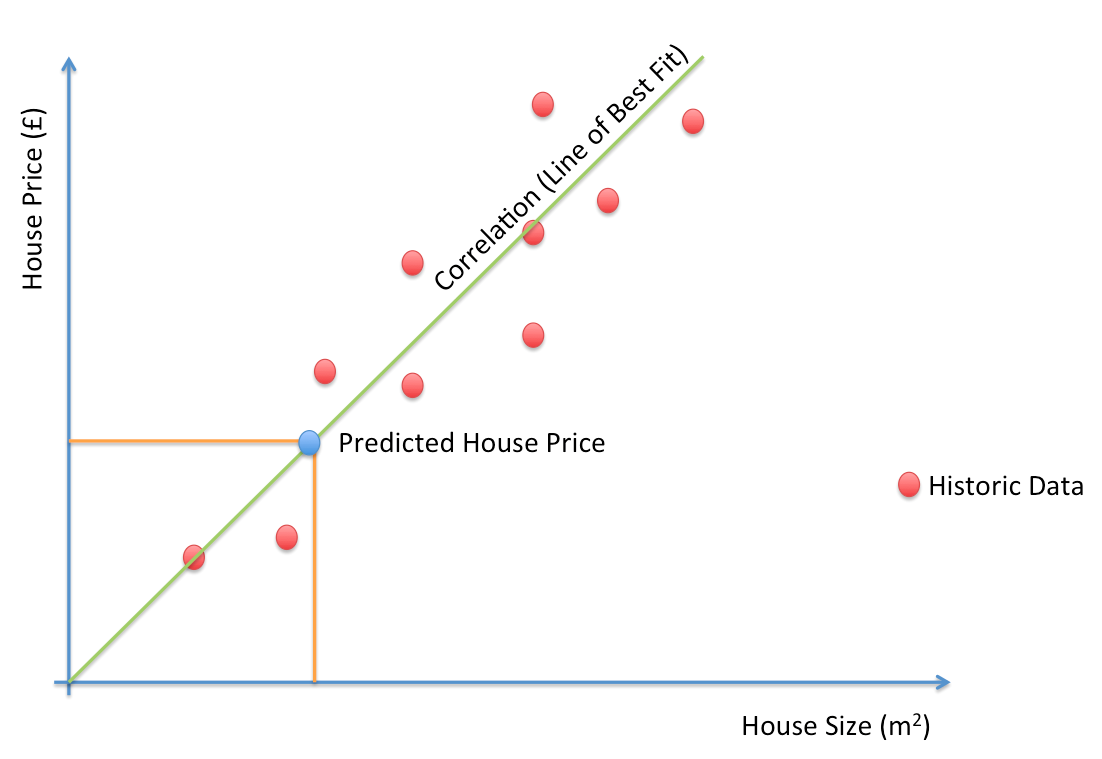
\includegraphics[height=8cm,keepaspectratio=true,clip=true]{imagenes/MarcoTeorico/regression_linear.png}
  \caption{Ejemplo Regresión (precio de una casa)}\label{Fig:regression}
\end{figure}

\item \textit{Problemas de Clasificación}: En un problema de clasificación, estamos tratando de predecir los resultados en una
salida discreta. En otras palabras, estamos tratando de asignar variables de entrada en categorías discretas. Algunos de los ejemplos son: clasificar perros o gatos determinando a que clase pertenece la imágen, evaluar si un email pertenece a la categoria "spam" o "no spam", entre otros.

\begin{figure}[H] \centering
  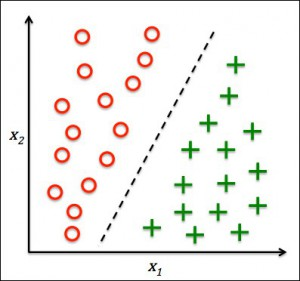
\includegraphics[height=8cm,keepaspectratio=true,clip=true]{imagenes/MarcoTeorico/classification.jpg}
  \caption{Ejemplo Clasificación}\label{Fig:clasificacion}
\end{figure}


\item \textit{Problemas de Aprendizaje no supervisado}: El aprendizaje no supervisado nos permite abordar los problemas con
poca o ninguna idea de cómo deben ser nuestros resultados. Podemos derivar la estructura de los datos donde no necesariamente conocemos el efecto de las variables. Podemos derivar esta estructura agrupando los datos basados en relaciones entre las variables en los datos. Con el aprendizaje no supervisado no hay una retroalimentación basada en los resultados de la predicción. El objetivo de problemas de aprendizaje no supervisados puede ser descubrir grupos de ejemplos similares dentro de los datos, donde se denomina agrupación (clustering), o determinar la distribución de datos dentro del espacio de entrada, conocida como estimación de densidad (density estimation), o proyectar los datos desde un espacio de nivel dimensional alto hasta dos o tres dimensiones con propósitos de visualización (Bishop, 2006).

\begin{figure}[H] \centering
  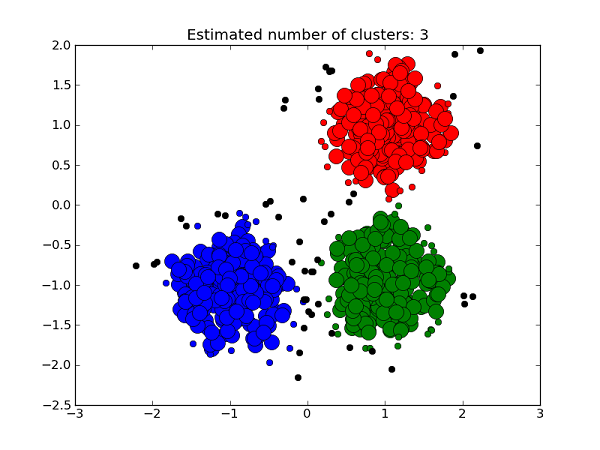
\includegraphics[height=8cm,keepaspectratio=true,clip=true]{imagenes/MarcoTeorico/claustering.png}
  \caption{Ejemplo aprendizaje no supervisado, claustering}\label{Fig:clauster}
\end{figure}
\end{itemize}

\subsubsection{Entrenamiento del modelo}
%https://docs.aws.amazon.com/es_es/machine-learning/latest/dg/training-ml-models.html
%clasificación supervisada metodos deduccion matematica


\subsubsection{Función de Costo}

\subsubsection{Algoritmos de Optimización}

\subsubsection{Validación de Modelos}
%Validación de Modelos (overfitting, underfitting)


\subsection{Computer Vision}

\subsection{Ajuste de Modelos}

\subsection{Redes Convolucionales}

\subsection{Regions Proposal}

\subsection{Clasificadores}







